\chapter{Neural variational message passing}

\section{Motivation}
Methods for Bayesian inference
often have a tradeoff between
efficiency and generality.
%Consider sampling algorithms:
%on one end of the spectrum we have
%Metropolis-Hastings
%which often scales poorly,
%but is extremely flexible, applying
%to almost any model.
%On the other end,
%we have Gibbs sampling
%which is more efficient, but 
%is restricted to conjugate models.
In variational inference,
general methods like black-box variational inference \cite{bbvi}
work in principle on any nonconjugate model,
but are less efficient
than specialized methods on certain models,
such as the variational autoencoder (VAE) \cite{vae}. 
Specialized
methods have the ability to
exploit structure in a model
that lends itself to efficient computation,
whereas general algorithms are often
unaware of this structure and lose out on the potential 
benefits.

The hope is to design an inference algorithm
that is both efficient and general,
and approaches to this problem have typically come in one of two forms.
The first is to make a general algorithm
aware of model-specific structure,
and to leverage it whenever possible.
The second is to take a specialized
algorithm and broaden its scope
by addressing its assumptions.
In this paper, we take the latter approach,
taking an algorithm
that is designed for conjugate models
and addressing how it fails in nonconjugate models.
Our resulting algorithm combines two powerful ideas 
in approximate inference: variational message
passing (VMP)\cite{vmp} and recognition networks.

%Variational inference for nonconjugate
%graphical models is difficult, but important.
%Many powerful nonconjugate probabilistic models such as
%non-linear dynamical
%systems, deep exponential families,
%and the variational autoencoder
%have exploded in popularity
%because of efficient and scalable inference algorithms.
%Designing such algorithms is tricky however,
%as the desire for an algorithm's generality can detract
%from its efficiency.

Conjugacy in models naturally lends itself
to efficient inference algorithms.
In many simple conjugate models,
we can compute the posterior distribution analytically.
But even in the general case, conjugacy is important
for efficient approximate inference.
This is best observed in mean-field variational inference
for graphical models, also called variational message passing (VMP) \cite{vmp}.
VMP is a simple, coordinate-ascent optimization of the
variational lower bound,
but its main drawback is its restriction
to conjugate-exponential models.

In many nonconjugate models,
however, efficient inference algorithms still exist.
Consider the VAE
and its structured variant (SVAE) \cite{svae}.
Both of these models
are highly nonconjugate, due to the inclusion
of a neural network observation model.
However, they address the nonconjugacy
by using neural networks, called recognition networks,
to help learn previously intractable posterior distributions.
Although VAE and SVAE utilize these networks
in subtly different ways, their purpose is the same: using
neural networks as function approximators
to make a previously intractable optimization feasible.

We thus propose neural variational message passing (NVMP),
a framework for nonconjugate variational inference
that generalizes use of recognition networks beyond
VAE and SVAE to a larger class
of nonconjugate models. 
As the name suggests,
NVMP is an extension of the
VMP framework, and while NVMP
generalizes VMP and SVAE, 
we still retain the modularity and
simplicity of VMP. 
We accomplish this by 
isolating the failure modes of VMP in nonconjugate models
and replacing previously intractable
computations with approximations
from recognition networks.

The paper is structured as follows. In \autoref{sec:background},
we derive the VMP algorithm, starting
with exponential families and conjugacy.
In \autoref{sec:nvmp},
we identify where VMP fails in nonconjugate
models and introduce the NVMP framework,
where we patch VMP's issues
with recognition networks.
We also provide
modifications to the NVMP framework
that integrate some newer ideas
in variational inference. 
Finally, in \autoref{sec:examples},
we provide several examples of how NVMP can
be easily applied to nonconjugate models, such
as sparse Bayesian linear regression
and a nonlinear dynamical system.

%VMP's original goal of modular
%inference
%in conjugate models lended itself to an intuitive software
%implementation, wherein models are specified
%graphically and inference is performed
%automatically afterwards.
%Likewise, NVMP enables a practical software
%implementation, where models need only be specified
%as one would write down any generative model. 
%Any conjugate structure 
%in the model is automatically exploited via VMP,
%and nonconjugacy is approximated
%by user-supplied recognition networks.

\subsection{Related Work}
The relevant works that inform this paper are
\cite{vmp} (VMP), \cite{vae} (VAE), and \cite{svae} (SVAE). 
VMP is a framework for variational inference
in CE models, but does
address nonconjugacy in some select situations,
relying on the Jaakola-Jordan trick \cite{jaakola}
and Monte-Carlo approximation.
In this work, we provide a more general way of extending VMP
to nonconjugate models, based on ideas
from VAE and SVAE. VAE and SVAE,
on the other hand, are models
where nonconjugacy is isolated to the observation model,
whereas in NVMP, we are not limited to this class of models.
Also related is \cite{ncvmp},
which is also a generalization of VMP.
It addresses nonconjugacy in VMP
by introducing a conjugate approximation
to the ELBO
that has the same gradients.
We also use a separate, tractable approximation
to the ELBO but rely on neural network
function approximation rather than matching gradients.

Several other works also
isolate the conjugacy in a model,
and address the nonconjugate component
by various means.
\cite{khan1} utilizes VMP
in conjugate components of the model, but stochastic
gradients in the nonconjugate components. This can in fact
be interpreted as a generalization of \cite{ncvmp}
but differs from NVMP in our use of recognition networks.
Perhaps the most similar work to ours
is \cite{khaaann}, which also utilizes recognition networks
alongside VMP.
The generalization of SVAE and VMP they provide is
is different from ours, however.
\cite{khaaann} uses recognition networks
with integrated graphical model structure.
whereas
we utilize recognition networks as local
function approximators.
Furthermore recognition
networks in \cite{khaaann} output model parameters,
amortizing inference in the process, in contrast with
NVMP recognition networks, which output potentials.

\section{Background}
\label{sec:background}

\subsection{Exponential families and conjugacy}

\begin{definition}
A probability distribution $p(x | \theta)$ is in the \textbf{exponential family}
if it can be written as
\begin{equation}
    \log p(x | \theta) = \left\langle t_x(x),\eta_x(\theta)\right\rangle - \log Z_x(\eta_x(\theta))
\end{equation}
where
\begin{enumerate}
    \item $\eta_x(\theta)$ is the \emph{natural parameter} function
    \item $t_x(x)$ is the \emph{sufficient statistic} function
    \item $\log Z_x(\eta_x(\theta))$ is the \emph{log partition} function
\end{enumerate}
\end{definition}


For a pair of random variables $x$ and $z$ and their
joint distribution $p(x, z) = p(x | z)p(z)$, we often say
they are conjugate if the posterior $p(z|x)$ is in the same
family as the prior $p(z)$. This definition
is useful when considering pairs of distributions,
but we aim to define conjugacy in a more global sense.

\begin{definition}
\label{def:conjugacy}
Consider a probabilistic model over several variables $p(x_1, \ldots, x_N) = \prod_{i = 1}^N p(x_i | \parents_{x_i})$ where $\parents_{x_i}$ are the parents of $x_i$.
We assume that each of these likelihoods $p(x_i | \parents_{x_i})$
is exponential family with sufficient statistics $t_{x_i}(x_i)$.
We define a model to be \textbf{conjugate-exponential} (CE)
if for each variable $x_i$ we can rewrite
the log-joint distribution as
\begin{equation}\label{eq:natparam}
    \log p(x_1, \ldots, x_N) \propto \left\langle t_{x_i}(x_i), \eta^*_{x_i}(\backslash x_i)\right\rangle
\end{equation}
where $\not{x_i}$ corresponds to all variables but $x_i$.
All occurrences of $x_i$ must be in $t_{x_i}(x_i)$ and the
joint distribution natural parameter $\eta^*_{x_i}(\not{x_i})$
contains all terms that are multiplied by the sufficient statistics of $x_i$.
\end{definition}
The previous, pairwise notion of conjugacy is captured by this definition 
by virtue of the fact that if two distributions
have matching sufficient statistics function, they are of the same family.

We now outline two properties of CE models
that will be important for VMP later on.
Consider a variable in a CE model $x_i$ with
parents $\parents_{x_i}$, children $\children_{x_i}$
and likelihood $p(x_i | \parents_{x_i})$.
\begin{property}
\label{prop:multilinear}
The natural parameter of $x_i$, $\eta_{x_i}(\parents_{x_i})$
can be expressed as a multilinear combination
of its parents' sufficient statistics, i.e.
\begin{equation}
    \eta_{x_i}(\parents_{x_i}) = f_{x_i}\left(\{t_p(p)\}_{p \in \parents_{x_i}}\right)
\end{equation}
where $f_{x_i}$ is some multilinear function for $x_i$.
\end{property}


%Consider a variable $x_i$ in a CE model.
%Extracting the joint distribution natural parameter 
%for a particular variable $x_i$
%can be done via a gradient with respect to $t_{x_i}(x_i)$.
%\begin{property}
%\label{prop:gradient}
%\begin{equation}
%    \eta^*_{x_i}(\not{x_i}) = \nabla_{t_{x_i}(x_i)} \log p(x_i, \not{x_i})
%\end{equation}
%This follows directly from \autoref{def:conjugacy}.
%\end{property}

\begin{property}
\label{prop:jointparam}
In a CE model,
the joint distribution natural parameter, $\eta^*_{x_i}(\not{x_i})$,
can be decomposed into summation of terms from $x_i$'s Markov blanket
(its children $\children_{x_i}$, parents $\parents_{x_i}$ and coparents).
\begin{equation}
\begin{split}
    &\eta^*_{x_i}(\not{x_i}) \\
    &= f_{x_i}\left(\{t_p(p)\}_{p \in \parents_{x_i}}\right)\\
    &+ \sum_{c \in \children_{x_i}} \nabla_{t_{x_i}(x_i)}\log p(c | x_i, \parents_{x_i} \not{x_i})\\
    &= f_{x_i}\left(\{t_p(p)\}_{p \in \parents_{x_i}}\right)
    + \sum_{c \in \children_{x_i}} \eta^c_{x_i}(x_i, \parents_c \backslash x_i)
\end{split}
\end{equation}
where $\parents_c \backslash x_i$ are the coparents of $x_i$ with respect to $c$.
The parents contribute one term to the natural parameter $f_{x_i}\left(\{t_p(p)\}_{p \in \parents_{x_i}}\right)$, along with one
term from each child $\eta^c_{x_i}(x_i, \parents_c \backslash x_i)$.

\end{property}
In general, these properties highlight the \emph{linearity} of terms
in CE models. The joint distribution natural parameter
is the sum of a multilinear function,
and several gradient terms.
This linearity is critical for the VMP derivation.


\subsection{Mean field variational inference}

Consider a latent variable model $p(\observed, \locals, \globals) = p(\globals)p(\locals | \globals)p(\observed | \locals, \globals)$
where $\observed=\{x_i\}_{i = 1}^N$ are observed data, $\locals =\{z_i\}_{i = 1}^N$ are
the local latent variables, and $\globals$ are the global latent variables.
In mean-field variational inference, 
the analytically intractable
posteriors $p(\locals, \globals|\observed)$ is approximated
by a variational distribution $q(\locals, \globals)$
which factorizes into individual distributions (factors), i.e.
$q(\locals, \theta) = q(\globals)\prod_{i = 1}^N q(z_i)$.

Variational inference proceeds by
maximizing the evidence lower bound (ELBO) $\L[q]$.
\begin{equation}
    \L[q] \triangleq \E_q\left[\log \frac{p(\observed, \locals, \globals)}{q(\locals, \globals)}\right]
\end{equation}
With a mean-field factorization of $q$, this optimization
breaks down into an individual optimization
over each variational factor. 
We will focus on a particular local latent variable $z_i$.
Although VMP does not distinguish between local latents
and global latents, the distinction will play a part in \autoref{sec:extensions}.
For $z_i$'s variational factor $q(z_i)$,
the ELBO is maximized by setting
\begin{equation}
    \log q^*(z_i) \propto \E_{q(\not{z_i})} \left[
    \log p(\observed, \locals, \globals)\right]
\end{equation}
where $q(\not{z_i})$ are all the variational factors excluding $q(z_i)$.
The dependence of $q^*(z_i)$ on the other factors leads
to a coordinate-ascent algorithm, where 
each $q(z_i)$ is updated with $q(\not{z_i})$ held constant,
iterating until
the ELBO has converged.

\begin{figure}[htp!]
    \centering
    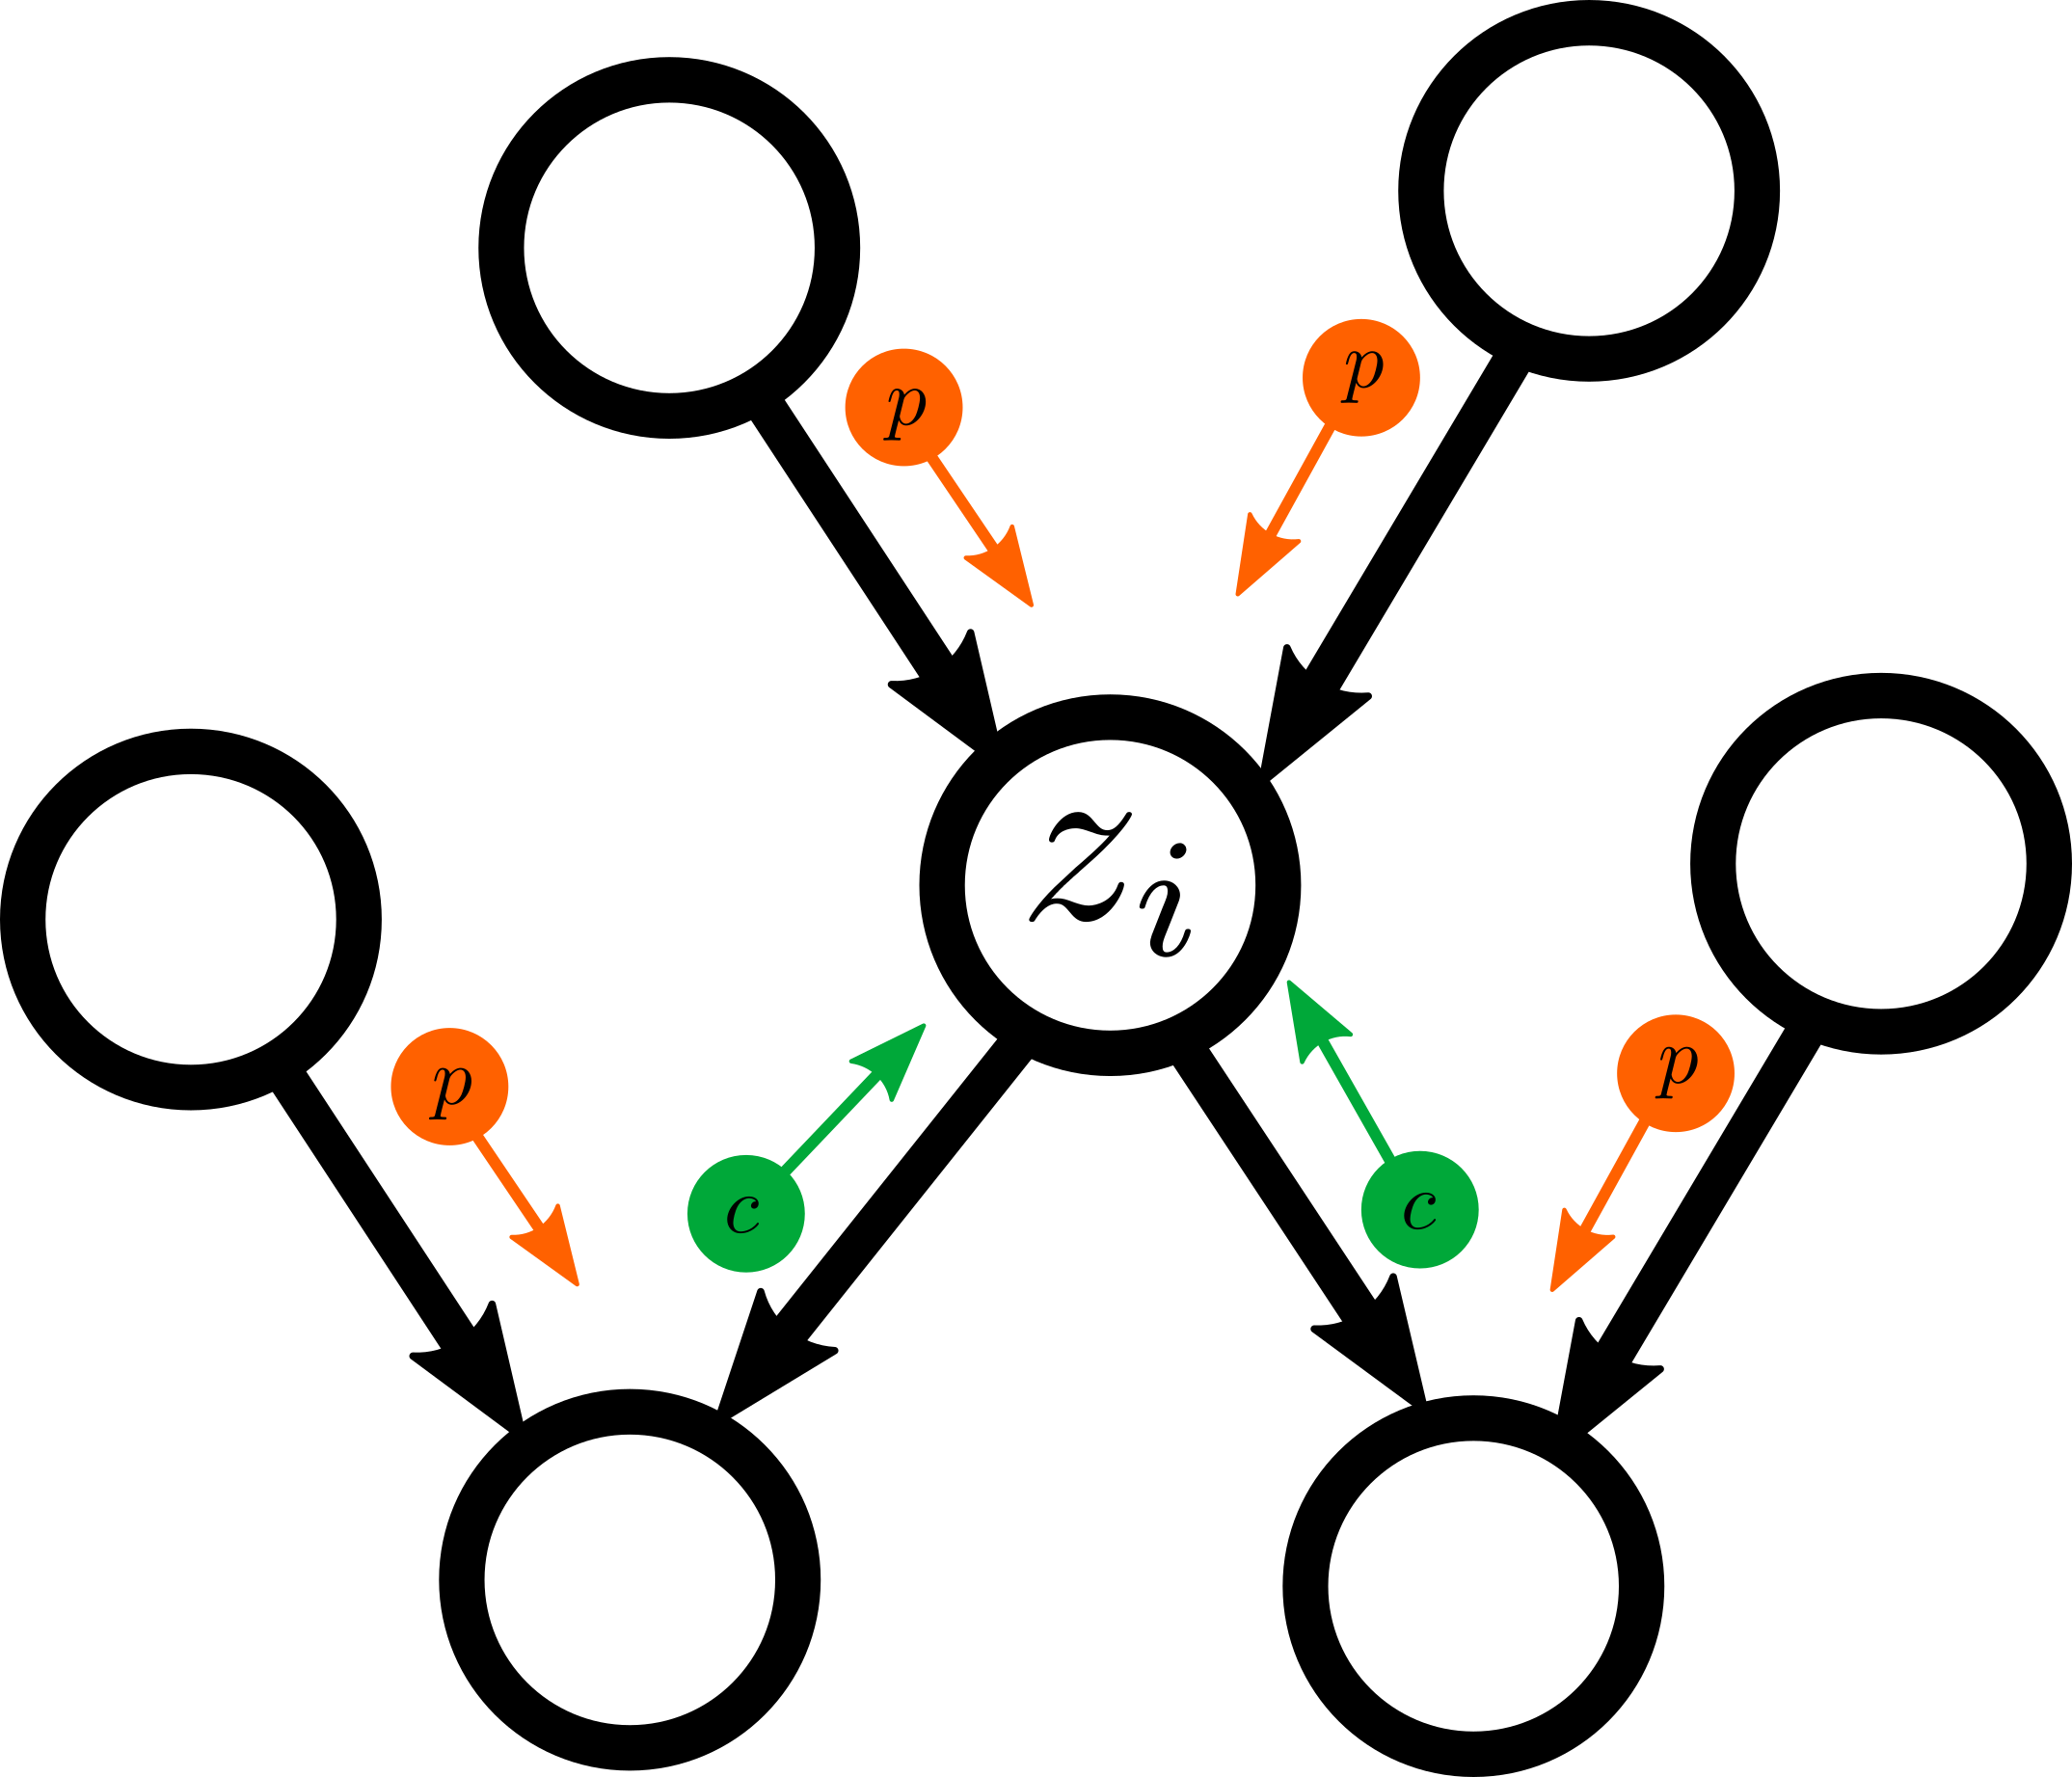
\includegraphics[width=0.4\textwidth]{img/nvmp/vmp-4}
    \caption{The messages that need to be computed in order to update
    node $z_i$ in variational message passing. Specifically, we require
    messages computed over the Markov blanket of $z_i$.}
    \label{fig:vmp}
\end{figure}
\begin{algorithm}[htp!]
\begin{algorithmic}
   \STATE {\bfseries Input:} data $X$, initial variational factors $q(z_i)$ for each latent variable $z$
   \REPEAT
   \FOR{each factor $q(z_i)$}
   \STATE Compute parent messages $\{\vmpmessage{p}{z_i}\}_{p \in \parents_{z_i}}$ (\autoref{eq:parentmessage})
   \STATE Compute coparent messages $\{\vmpmessage{v}{c}\}_{c \in \children_{z_i}, v \in \parents_c \backslash z}$ (\autoref{eq:parentmessage})
   \STATE Compute child messages $\{\vmpmessage{c}{z_i}\}_{c \in \children_{z_i}}$
   (\autoref{eq:childmessage})
   \STATE $\eta^q_{z_i} \leftarrow f_{z_i}\left(\{\vmpmessage{p}{z_i}\}_{p \in \parents_{z_i}}\right) + \sum_{c \in \children_{z_i}} \vmpmessage{c}{z_i}$ 
   \ENDFOR
   \UNTIL{ELBO has converged}
\end{algorithmic}
   \caption{Variational message passing}
   \label{alg:vmp}
\end{algorithm}


In a conjugate-exponential model, we can utilize the definition
of conjugacy to further simplify the optimization of $q^*(z_i)$.
\begin{equation}
\begin{split}
    \log q^*(z_i) &\propto \E_{q(\not{z_i})} \left[
    \log p(\observed, \locals, \globals)\right]\\
    &\propto \E_{q(\not{z_i})} \left[
    \left\langle t_{z_i}(z_i), \eta^*_{z_i}(\not{z_i})\right\rangle\right]\\
    &= 
    \left\langle t_{z_i}(z_i), \E_{q(\not{z_i})}\left[\eta^*_{z_i}(\not{z_i})\right]\right\rangle
\end{split}
\end{equation}
Thus, $q^*(z_i)$ 
is in the same family as $p(z_i | \parents_{z_i})$,
as the sufficient statistic functions match,
and has natural parameter $\eta^q_{z_i} \triangleq \E_{q(\not{z_i})}\left[\eta^*_{z_i}(\not{z_i})\right]$.

\subsection{Variational message passing}

Variational message passing provides a modular way of
computing
an optimal latent factor $q^*(z_i)$
in terms of its local graphical model structure.
Specifically, we utilize \autoref{prop:jointparam}
to further pass in the expectation.
\begin{equation}
\begin{split}
    \eta^q_{z_i} &= \E_{q(\not{z_i})}\left[\eta^*_{z_i}(\not{z_i})\right] \\
                 &= f_{z_i}(\{\E_{q(\not{z_i})}\left[t_p(p)\right]\}_{p \in \parents_{z_i}}) \\
                 &+ \sum_{c \in \children_{z_i}} 
         \nabla_{t_{z_i}(z_i)} \E_{q(\not{z_i})}\left[\log p(c | z_i, \parents_{c} \backslash z_i)\right]
\end{split}
\end{equation}

This decomposition leads to a message passing algorithm, where
the natural parameter $\eta^q_{z_i}$
can be computed as the sum of messages from the children and parents.
\paragraph{Parent message:}
The message from a parent $p$ to $z_i$ is
\begin{equation} \label{eq:parentmessage}
    \vmpmessage{p}{z_i} = \E_{q(p)}\left[t_p(p)\right]
\end{equation}

\paragraph{Child message:}
The message from child $c$ to $z_i$ is

\begin{equation} \label{eq:childmessage}
    \vmpmessage{c}{z_i} = \nabla_{t_{z_i}(z_i)} \E_{q(c, \parents_{c} \not{z_i})}\left[\log p(c | z_i, \parents_{c} \not{z_i})\right]
\end{equation}
Computing the gradient in the child message involves
computing messages from the coparents of $z_i$ with respect to $c$ in order to evaluate the expectation.
After all relevant messages
have been computed, the natural parameter is $q^*(z_i)$ calculated as
\begin{equation}
    \label{eq:vmpparam}
   \eta^q_{z_i} = f_{z_i}\left(\{\vmpmessage{p}{z_i}\}_{p \in \parents_{z_i}}\right) + \sum_{c \in \children_{z_i}} \vmpmessage{c}{z_i}
\end{equation}

An important note is that if a node corresponds to observed data,
expectations over the node are replaced with the empirical quantity.
The complete VMP algorithm is described in \autoref{alg:vmp} and
a diagram of the necessary messages for updating a node
is shown in \autoref{fig:vmp}.

\section{Neural variational message passing}
\label{sec:nvmp}

In this section, we examine
the assumptions that the VMP derivation makes
and identify where recognition networks
can assist in inference.

\iffalse
VMP relies on the CE assumption that
for each variable $z_i$, the sufficient statistics
of its likelihood $t_{z_i}(z_i)$ are the same
sufficient statistics present in the joint distribution
over all variables. 
This property ensures that the optimal
variational distribution for a latent variable
will be in the same family of that latent variable's likelihood.
However, suppose there are statistics in the joint density
that do not match a simple exponential family. Consider
the variational autoencoder, which has a neural network
in the generative model. Neural networks will produce
naturally complicated statistics of latent variables 
in the joint density, so attempting to rewrite terms
to match, say a Gaussian posterior distribution,
will be impossible.
\fi

In NVMP we first
assume variational posteriors that match
the likelihood, that is $q(z_i)$ will
be the family as $p(z_i | \parents_{z_i})$. 
This step 
is quite common in variational inference
as even in conjugate
models, the true posterior of a latent variable may not belong
in the same family as its likelihood.
Where NVMP differs is in how latent variational factors
are optimized.
NVMP uses VMP messages whenever possible,
but when VMP messages are not possible due to 
nonconjugacy, they are replaced with NVMP messages,
$m^{\text{NVMP}}_{p \rightarrow z},m^{\text{NVMP}}_{c \rightarrow z}$.
We now derive the form of these modified messages.

\paragraph{Parent message:}
Consider \autoref{prop:multilinear}:
if $f_{z_i}$ is not multilinear in the sufficient statistics of one of
its parents
parents $p$,
we can no longer compute the natural parameter
from $\vmpmessage{p}{z_i}$.
However, we can perform a Monte Carlo approximation of $f_{z_i}$.
Thus, in NVMP, if we $f_{z_i}$ is no longer
multilinear in the sufficient statistics of its parents,
we approximate $f_{z_i}$ using samples from $q(p)$.
\footnote{Note that we can use multiple samples from $q(p)$ for a better Monte Carlo
approximation.}

\begin{equation}
    m^{\text{NVMP}}_{p \rightarrow z} = p'
\end{equation}

\paragraph{Child message:}
Nonconjugate models result in intractable child messages.
The entire strategy of re-arranging
the log-likelihood
in terms of sufficient statistics $t_{z_i}(z_i)$ to eventually
take a gradient is infeasible.
However, adapting the approach of SVAE allows us to
compute the child message for an approximation of the ELBO.
In conjugate-exponential models, utilizing \autoref{prop:jointparam},
we are able to rewrite
\begin{equation}
\log p(c | z_i, \parents_c \not{z_i}) \propto \left\langle t_{z_i}(z_i), \eta_{z_i}^c(c, \parents_c \not{z_i})\right\rangle 
\end{equation}
and $\E_{q(\backslash z_i)}\left[\eta_{z_i}^c(c, \parents_c \not{z_i})\right]$
would be the corresponding message $\vmpmessage{c}{z_i}$.
If we are unable to arrange $\log p(c | z_i, \parents_c \not{z_i})$ in this way, we approximate this log-likelihood with a factor $\psi(c, z_i, \parents_{c} \not{z_i}; \phi)$, as done in \cite{svae}.
\begin{equation}
\label{eq:rectrick}
\begin{split}
\log p(c | z_i, \parents_c \not{z_i}) &\approx \psi(c, z_i, \parents_{c} \not{z_i}; \phi) \\
\end{split}
\end{equation}
We choose a particular form of $\psi$ that results in an easy optimization
of an approximate ELBO.
\begin{equation}
\begin{split}
    \psi(c, z_i, \parents_{c} \not{z_i}; \phi) &\triangleq \left\langle t_{z_i}(z_i), r^{c \rightarrow z_i}_{\phi}(c, \parents_{c} \not{z_i})\right\rangle
\end{split}
\end{equation}
where $r_{\phi}$ is a recognition network parameterized by $\phi$.
Following the original steps in VMP
and computing the gradient of the approximate log-likelihood
with respect to $t_{z_i}(z_i)$ results in a new message.
\begin{equation}
    \E_{q(c)q(\parents_c \backslash z_i)} \left[r^{c \rightarrow z_i}_{\phi}(c, \parents_{c}\not{z_i})\right]
\end{equation}
This expectation can be approximated via a Monte Carlo sample $c' \sim q(c)$
and NVMP messages from the coparents (which are also Monte Carlo samples).
\footnote{As in the parent message case, our Monte Carlo approximation can
be improved with multiple samples.}

\begin{equation}
    \nvmpmessage{c}{z_i} = r^{c\rightarrow z_i}_{\phi}\left(
    c', \{\nvmpmessage{v}{z_i}\}_{v \in \parents_c \not{z_i}}\right)
\end{equation}

The NVMP child message for child $c$ passes Monte Carlo samples
of $c$ and of $z_i$'s coparents into a recognition network.
Note that this strategy assigns a recognition
network to \emph{each} nonconjugate edge
in a graph. However, in practice,
it would be prudent to share parameters
across networks
whenever possible,
especially for edges where nodes are sampled
independently (e.g. IID data).
Finally, we can compute the parameter for $q^*(z_i)$
as before, but instead of using $f_{z_i}$, we use $z_i$'s
exponential family natural parameter function $\eta_{z_i}(\parents_{z_i})$.
\begin{equation}
    \label{eq:nvmpparam}
   \eta^q_{z_i} = \eta_{z_i}\left(\{\nvmpmessage{p}{z_i}\}_{p \in \parents_{z_i}}\right) + \sum_{c \in \children_{z_i}} \nvmpmessage{c}{z_i}
\end{equation}
These message definitions are a drop-in replacement
for messages in VMP, allowing us to re-use \autoref{alg:vmp},
using NVMP messages whenever possible. The only
difference is that we use \autoref{eq:nvmpparam} to compute
the natural parameter instead of \autoref{eq:vmpparam}.
Importantly, introducing recognition networks
into the VMP framework does mean we are no longer
directly optimizing the ELBO. However, we will
show that we are still optimizing a lower
bound on the ELBO, and if the recognition networks
have high enough capacity, the bound is tight.

\subsection{Learning recognition network weights}
The final step is learning recognition network
weights and other model parameters.
In the inner loop of NVMP, we
iterate message passing to convergence.
This outputs a set of optimal variational
factors, conditioned on the recognition networks.
We then take a gradient step
to maximize the ELBO.
In a nonconjugate model, the ELBO isn't
directly computable due to intractable expectations.
Therefore, 
recognition networks and model parameters are optimized
via stochastic gradients of the ELBO using samples from $q$.
In a latent variable model, this would correspond to 
taking gradients of
\begin{equation}
    \L[q] \approx \frac{1}{L}\sum_{l = 1}^L \log \frac{p(\observed, \locals^{(l)}, \globals^{(l)})}{q(\locals^{(l)}, \globals^{(l)})}
\end{equation}
The reparametrization trick should be utilized whenever possible,
to reduce the variance of the gradients \cite{vae}.
Furthermore, the gradients with respect recognition networks
and model parameters computed using optimal variational
distributions, meaning we must backpropagate through
the iterative process to compute the gradients.

\subsection{Lower-bounding the ELBO}
The inclusion of recognition networks
in the local optimization for each factor
induces a global
optimization on a lower bound the ELBO. 

\begin{theorem}
\label{thm:lowerbound}
The NVMP algorithm optimizes a lower bound on the ELBO.
\begin{proof}
 (sketch) Each individual coordinate ascent update optimizes its own lower bound on the ELBO. Thus, holistically, NVMP optimizes a lower bound on the ELBO by optimizing individual lower bounds. We refer you to the supplement for the full proof.
\end{proof}
\end{theorem}

\subsection{Extensions to NVMP}
\label{sec:extensions}

NVMP is a fully-specified template 
for nonconjugate inference, but in practice,
some modifications are useful. In this section,
we outline ways some recent
developments in variational inference which naturally fit
into the NVMP framework.

Stochastic variational inference (SVI), or stochastic VMP, is
a strategy to adapt mean-field variational inference
to large datasets \cite{svi}. As datasets
have grown larger, we typically require
algorithms that operate on mini-batches
of data to scale and SVI adds this functionality to VMP. 
SVI enables computing natural gradients of the ELBO for parameters in our model.We detail integrating SVI into NVMP in the supplement.

%\subsection{Amortized inference}
%\label{sec:amortized}

Amortized inference enables neural networks
to directly act as posterior distributions, as in VAE, as opposed to outputting approximate messages, as in SVAE. When we want a black-box approximate posterior, learning such a recognition network can be useful in downstream inference tasks. We detail how 
amortized inference networks can be used with NVMP in the supplement.

\section{Examples and experiments}
\label{sec:examples}

In this section, to show the simplicity by
which NVMP can be used for nonconjugate inference,
we provide several example models 
where NVMP messages can be used, and some simple
experiments. We do not aim to outperform
similar frameworks, but rather to show the versatility of NVMP, as NVMP works on models ranging from the VAE to Bayesian logistic regression.
The graphical models are pictured in \autoref{fig:graphicalmodels},
and in all experiments, we utilized the stochastic variant
of NVMP, and did not use amortized inference.

\subsection{Bayesian linear regression with a sparse prior}

In the Bayesian lasso variant of sparse linear regression.
we put an exponential prior on the variance of our weights $w$ \cite{bayesianlasso}.

\begin{figure*}
    \centering
    \begin{subfigure}[t]{0.19\textwidth}
        \centering
        \includegraphics{tikz/representation/nvmp/lr-prior}
        \caption{Bayesian linear regression with a sparse prior}
    \end{subfigure}
    \hfill
    \begin{subfigure}[t]{0.19\textwidth}
        \centering
        \includegraphics{tikz/representation/nvmp/blr}
        \caption{Bayesian logistic regression}
    \end{subfigure}
    \hfill
    \begin{subfigure}[t]{0.19\textwidth}
        \centering
        \includegraphics{tikz/representation/nvmp/vae}
        \caption{Variational autoencoder}
    \end{subfigure}
    \begin{subfigure}[t]{0.19\textwidth}
        \centering
        \includegraphics{tikz/representation/nvmp/svae-gmm}
        \caption{SVAE-GMM}
    \end{subfigure}
    \begin{subfigure}[t]{0.19\textwidth}
        \centering
        \includegraphics{tikz/representation/nvmp/nlds}
        \caption{Nonlinear dynamical system}
    \end{subfigure}
    \caption{Five nonconjugate models in which NVMP messages can be used for approximate inference.}
    \label{fig:graphicalmodels}
\end{figure*}

\begin{align*}
    \sigma_w^2 &\sim \text{Exponential}([1, \ldots, 1]) \\
    w | \sigma^2_w &\sim \N(0, \text{diag}\left(\sigma_w^2)\right) \\
    y_i | w, x_i &\sim \N(w^Tx_i, \sigma^2_y)
\end{align*}

Exact posterior inference in this model is not tractable, due
to the exponential prior, so approximation is necessary. 
Since $y_i$ is conjugate to $x_i$ and $w$, we still use
the VMP messages $\vmpmessage{x_i}{y_i}, \vmpmessage{y_i}{w}, \vmpmessage{w}{y_i}$,
but otherwise we use NVMP messages $\nvmpmessage{w}{\sigma_w^2}, \nvmpmessage{\sigma_w^2}{w}$. We require one recognition
network $r_{\phi}^{w \rightarrow \sigma^2_w}(w)$, which produces the message $\nvmpmessage{w}{\sigma_w^2}$.

\paragraph{Experiment} We performed NVMP with this model on the
Boston housing regression dataset \cite{uci}.
We utilized a 2-layer 500-wide feedforward network with Tanh activations
as $r_{\phi}^{w \rightarrow \sigma^2_w}(w)$.
Regular linear regression learns weights with $\|w\|_1 = 25.56$
and testing mean squared error $33.45$.
Lasso regression learns weights with $\|w\|_1 = 3.27$ 
and testing mean squared error $41.07$.
NVMP learns a weight vector with $\|w\|_1 = 7.31$
and testing mean squared error $35.60$.
The Bayesian lasso learns a sparsity
in between unregularized regression and lasso,
consistent with findings in \cite{bayesianlasso},
which uses a Gibbs sampler to perform inference in the model.

\subsection{Bayesian logistic regression}

Bayesian logistic regression is a model for binary classification
of data and labels $\{x_i, y_i\}_{i = 1}^N$.
\begin{align*}
    w &\sim \N(0, I) \\
    y_i | w, x_i &\sim \text{Bernoulli}(\sigma(w^Tx_i))
\end{align*}

The approximated messages are $\nvmpmessage{x_i}{y_i}, \nvmpmessage{w}{y_i}, \nvmpmessage{y_i}{w}$ with recognition network $r_{\phi}^{y_i \rightarrow w}(x_i, y_i)$.

\paragraph{Experiment} We ran a simple experiment, performing
NVMP with this model on MNIST restricted to the 3 and 8 digit.
We utilized a 2-layer 500-wide feedforward network with Tanh activations
as $r_{\phi}^{y_i \rightarrow w}(x_i, y_i)$.
Traditional logistic regression achieves a test set accuracy of 95.6\%
and our method achieves 95.1\%. This is drop in accuracy is likely due to the
prior, as running NVMP without the prior
also results in an accuracy of 95.6\%.

\iffalse
\subsection{Variational autoencoder}
The variational autoencoder \cite{vae} generates data
by first sampling data from a simple Gaussian prior
and then passing it through a neural network.

\begin{align*}
    x_i &\sim \N(0, I) \\
    y_i | x_i &\sim \N(\mu_\gamma(x_i), \Sigma_\gamma(x_i))
\end{align*}
where $\mu_\gamma$ and $\Sigma_\gamma$ are a neural network parameterized
by weights $\gamma$.

With NVMP, we use approximate messages
$\nvmpmessage{x_i}{y_i}$, and
$\nvmpmessage{y_i}{x_i}$, with a 
single recognition network $r_\phi^{y_i \rightarrow x_i}(y_i)$.

It is important to note the difference between the
inference algorithm for VAE as originally specified
and inference with NVMP. The recognition network in VAE outputs 
the parameters of $q(x_i | y_i)$ directly,
whereas in NVMP, the parameters of $q(x_i | y_i)$
are the sum of the output of the recognition network $r_\phi^{y_i \rightarrow x_i}(y_i)$
and the natural parameter of the prior on $x_i$.
We omit running an experiment for this model, due to NVMP's similarity
to the AEVB algorithm. In fact, using amortized inference
will result in the exact VAE inference algorithm.
\fi

\subsection{SVAE-GMM}
The structured variational autoencoder Gaussian mixture model (SVAE-GMM) \cite{svae} learns representations
that have a latent cluster structure.
It accomplishes this by attaching a neural network observation model
to a Gaussian mixture model.
\begin{align*}
    \{\mu_k, \Sigma_k\}_{k = 1}^K &\sim \NIW(\Psi, \nu, \mu_0, \kappa) \\
    \pi &\sim \text{Dirichlet}(\alpha) \\
    z_i | \pi &\sim \text{Categorical}(\pi) \\
    x_i | z_i, \{\mu_k, \Sigma_k\} &\sim \N(\mu_{z_i}, \Sigma_{z_i}) \\
    y_i | x_i &\sim \N(\mu_\gamma(x_i), \Sigma_\gamma(x_i))
\end{align*}
where $\mu_\gamma$ and $\Sigma_\gamma$ are a neural network parameterized by $\gamma$.

Our NVMP messages are $\nvmpmessage{x_i}{y_i}, \nvmpmessage{y_i}{x_i}$
and the rest remain VMP messages. We also omit an experiment
for this model, as stochastic NVMP
results in the same inference algorithm as described in \cite{svae},
without the prior on neural network observation model weights.

\subsection{Nonlinear dynamical system}
Consider a dynamical system that evolves
according to a neural
network transition function, but is observed with Gaussian noise:
\begin{align*}
    x_{t + 1} | x_t &\sim \N(\mu_\gamma(x_t), \Sigma_\gamma(x_t)) \\
    y_t | x_t &\sim \N(x_t, \sigma^2_yI)
\end{align*}
where $\mu_\gamma$ and $\Sigma_\gamma$ are a neural network parameterized by $\gamma$.

In this model, we require NVMP messages $\nvmpmessage{x_{t + 1}}{x_t}, \nvmpmessage{x_t}{x_{t + 1}}$ with a recognition network $r^{x_{t + 1} \rightarrow x_t}_\phi(x_{t + 1})$.

\begin{figure}
    \centering
    \includegraphics[width=0.3\textwidth]{img/nvmp/nlds}
    \caption{A learned ``circular'' dynamics system using NVMP.}
    \label{fig:nlds}
\end{figure}

\paragraph{Experiment} We simulated a nonlinear dynamical system
with 2-dimensional data and a transition function
that moves points along a circle centered at the origin.
We utilized 2-layer 500-wide feedforward networks with Tanh activations
for both $r^{x_{t + 1} \rightarrow x_t}_\phi(x_{t + 1})$ and $\mu_\gamma, \Sigma_\gamma$.
Pictured in \autoref{fig:nlds} is the learned neural network dynamical system.
It learns the circular pattern the data is generated from, indicating
that NVMP successfully fit a transition function.

%\subsection{Recurrent switching linear dynamical system}
%The recurrent switching linear dynamical system, introduced
%in \cite{rslds},
%We consider a switching linear dynamical system
%where we have hidden states that evolve Markovian
%with a non-linear dependence on observation.
%
%Our model for dataset $\{x^{(i)}_0, x^{(i)}_1, \ldots, x^{(i)}_T\}_{i = 1}^N$
%is
%\begin{align*}
%    \pi^0 &\sim \mathrm{Dir}(\alpha) \\
%    \{\pi_k\}_{k = 1}^K &\sim \mathrm{Dir}(\alpha) \\
%    \{A_k, \Sigma_k\}_{k = 1}^K &\sim \MNIW(\Psi, M_0, V, \nu) \\
%    x_0 &\sim \N(\mu_0, \Sigma_0) \\
%    s_0 &\sim \mathrm{Cat}(\pi^0) \\
%    s_{t + 1} | s_t, x_t &\sim \mathrm{Cat}(f(\pi_{s_t}, g_\gamma(x_t)) \\
%    x_{t + 1} | s_{t + 1}, x_t, \{A_k, \Sigma_k\}_{k = 1}^K &\sim \N(A_{s_{t + 1}}x_t, \Sigma_{s_{t + 1}})
%\end{align*}
%
%This model is fully conjugate other than the non-linear state transition.
%Specifically, we have a neural network $g_\gamma$ which outputs
%potentials to the state transition distribution. $f$ is a function
%that normalizes the sum of the potentials and the Markovian transition
%probabilities $\pi_{s_t}$.
%
%We can learn this model with NVMP by approximating
%the message $m_{s_{t + 1} \rightarrow s_t} = r_\phi(\eta_{s_t}, x_t)$.
%In this scenario, we share neural network weights $\phi$
%between all nonconjugate messages, since there is one for each time
%step in this model.

\section{Discussion}
We have written a software package,
built on top of Tensorflow. The package
was designed to make modeling as easy as possible.
NVMP enables specifying models purely in
the forward direction, like in Edward and Stan.
Rather than using a black-box method
or sampling afterwards,
NVMP requires recognition networks
as inputs to the algorithm
wherever necessary. After this, inference
is completely automated and efficient, relying on
GPU computations through the Tensorflow computational graph.

A key limitation of NVMP 
(and other models that utilize recognition networks)
is that gradients with respect to model parameters
must only include continuous random variables,
as backpropagation through discrete random
variables is not possible. However, integrating 
the Gumbel-Softmax trick or modifications
such as those in 
\cite{dvae} and \cite{ndrl} into NVMP is a promising
step forward in addressing this concern.